\begin{figure}[h] 
\centering 
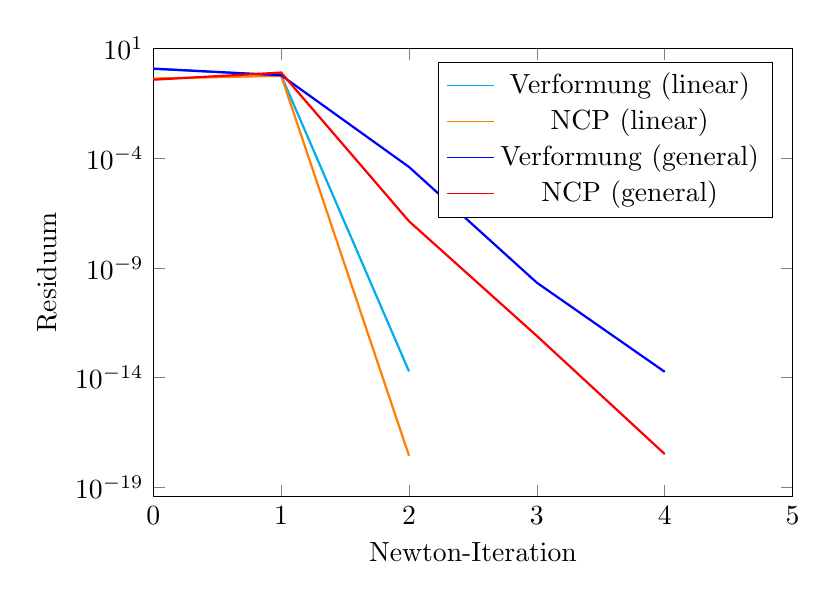
\begin{tikzpicture}[every plot/.append style={thick}] 
\begin{axis}[ 
label style={font=\normalsize}, 
xlabel={Newton-Iteration}, 
ylabel={Residuum}, 
xmin=0, xmax=5, 
ymode=log, 
ymin=0, ymax=10, 
width=0.8\textwidth, 
height=0.6\textwidth, 
legend pos=north east, 
legend style={cells={align=left}}, 
grid style=dashed, 
] 
\addplot[ 
color=cyan, 
] 
coordinates { 
(0, 1.15e+00)(1, 5.74e-01)(2, 1.93e-14)}; 
\addlegendentry{Verformung (linear)} 
\addplot[ 
color=orange, 
] 
coordinates { 
(0, 4.15e-01)(1, 5.52e-01)(2, 2.79e-18)}; 
\addlegendentry{NCP (linear)} 
\addplot[ 
color=blue, 
] 
coordinates { 
(0, 1.17e+00)(1, 5.83e-01)(2, 3.90e-05)(3, 2.10e-10)(4, 1.84e-14)}; 
\addlegendentry{Verformung (general)} 
\addplot[ 
color=red, 
] 
coordinates { 
(0, 3.66e-01)(1, 7.74e-01)(2, 1.32e-07)(3, 7.91e-13)(4, 3.33e-18)}; 
\addlegendentry{NCP (general)} 
\end{axis} 
\end{tikzpicture} 
\caption{Residuen des Stoffgesetzes 'Linear elastisch' mit Hinderniss 'Parabel' und 2178 Freiheitsgraden für die Verschiebung.} 
\label{fiq:Linearelastisch_Parabel_level4} 
\end{figure} 
